\scanpage{7}\mspage{4.}
\begingroup
\makeatletter\tagsleft@true\makeatother
4. \uline{The} \uline{canonical} \uline{filtration} \uline{on} \uline{the} \uline{group} of $v$-\uline{adic} \uline{points}. Let $F(x,y)-y^2+a_1xy+\ldotp$ be a minimal equation for $E$ relative to a valuation $v$. Let $\widetilde F(x,y)$ be the reduction of $F$ $(\bmod\,\mathfrak{p})$ and let $\widetilde E$ denote the plane cubic $\widetilde F=0$ defined over the residue field $k$. By Theorem 3.2, $\widetilde E$ is uniquely determined by $E$ up to a projective transformation of the form (2.1) over $k$: Let $\widetilde E_0$ denote the non-singular part of $\widetilde E$. Then $\widetilde E_0$ is an algebraic group with origin $\widetilde O$. (If $\widetilde E$ is non singular, then $\widetilde E_0-\widetilde E$ is an elliptic curve, If $\widetilde E$ has a node
\parbox[c]{1.4em}{\setlength{\topsep}{0pt}\figure{
\begin{tikzpicture}[x=0.95em,y=0.95em]
\draw[line width=.8pt,line cap=round] (0.97,.01) .. controls (.73,.19) and (.45,.66) .. (.24,.64) .. controls (.01,.65) and (-.02,.30) .. (.12,.16) .. controls (.29,.02) and (.49,.18) .. (.60,.34) .. controls (.76,.52) and (.85,.69) .. (.96,.87);
\end{tikzpicture}}}, then $\widetilde E_0\approx\mathbb{P}^1-(\text{two points})$ is a multiplicative group, and if $\widetilde E$ has a cusp
\parbox[c]{1.4em}{\setlength{\topsep}{0pt}\figure{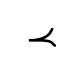
\begin{tikzpicture}[x=0.95em,y=0.95em]
\draw[line width=.9pt,line cap=round] (.91,.66) .. controls (.81,.40) and (.59,.24) .. (.02,.22) .. controls (.61,.23) and (.87,.25) .. (1.01,.02);
\end{tikzpicture}}}, then $\widetilde E_0=\mathbb{P}^1-(\text{one point})$ is an additive group; here We have ignored questions of rationality, but if $k$ is perfect, so that the singularity of $\widetilde E$ is rational over $k$, then the analysis is the same, except that in case of a node, $\widetilde E_0$ is a multiplicative group ``twisted'' by the quadratic extension obtained by adjoining to $k$ the two tangents at the node)

Let $E(K)$ denote the group of points on $E$ rational over $K$, and let $\rho:E(K)\longrightarrow\widetilde E(k)$ denote the reduction map (defined naively in terms of the given projective coordinates --- by Theorem 3.2 it is independent of the coörds.) Let $E_0(K)=\rho^{-1}(\widetilde E_0(k))$ be the set of points whose reduction is non-singular.

\uline{Theorem 4.1}: $E_0(K)$ \uline{is} \uline{a} \uline{subgroup} \uline{of} \uline{finite} \uline{index} \uline{in} $E(K)$, \uline{and} $\rho_0:E_0(K)\to\widetilde E_0(k)$ \uline{is} \uline{a} \uline{homomorphism} \uline{of} \uline{groups}.

A straightforward but tedious proof can be given, using the addition formulae, for everything except the `finite index''. That finiteness depends on the minimality of the equation, and a proof of finiteness is implicit in the algorithm for reducing to minimal form given below.

We denote the kernel of $\rho_0$ by $E_1(K)$; it consists of the points $P=(x,y)$ in $E(K)$ such that $v(x)<0$ and $v(y)<0$. Clearly, from \unsure{(1 1)|(1.1)} since $v(a_i)\geqslant0$, we have $v(x)<0\Longleftrightarrow v(y)<0$, in which case $v(x)=-2m$ and $v(y)=-3m$ for some $m$. For each $m\geqslant1$ we let $E_m(K)=\{(x,y)\in E(K)\mid v(x)\leq-2m\ \text{and}\ v(y)\leq-3m\}$ (understanding of course that $O\in E_m(K)$ for all $m$).

\uline{Theorem 4.2}: \uline{Let} $z=-\dfrac{x}{y}$. \uline{Then} $z$ \uline{is} \uline{a} \uline{uniformising} \uline{parameter} \uline{at} $O$. \uline{The} \uline{expansions}
\begingroup\scriptsize
\[
\begin{aligned}
x&=z^{-2}-a_1z^{-1}-a_2-a_3z-(a_4+a_1a_3)z^2
 -\ldotp\,\ldotp\,\ldotp\,\ldotp\\
y&=-z^{-1}x=-z^{-3}+a_1z^{-2}+a_2z^{-1}+a_3+(a_4+a_1a_3)z+\ldots\\
\omega&=dt\bigl(1+a_1t+(a_1^2+a_2)t^2+(a_1^3+2a_1a_2+a_3)t^3+
 (a_1^4+3a_1^2a_2+6a_1a_3+a_2^2+2a_4)t^4+\ldotp\,\unsure{-|\ldotp}
\end{aligned}
\tag*{(4.3)}
\]
\endgroup
\uline{have} \uline{coefficients} \uline{in} $R$. \uline{So} \uline{also} \uline{does} \uline{the} \uline{formal}
\deleted{$(\unsure{a_1^4+3a_1^2a_2}+6a_1\unsure{a_3}\unsure{+a_2^2+2a_4})\unsure{t^4}$}
\uline{group} \uline{law} $\Phi(Z_1,Z_2)=Z_1+Z_2+\ldotp\,\ldotp\,\ldotp\,\ldotp$ \uline{defined} \uline{by} \uline{the} \uline{equation} $z(P+Q)=\Phi(z(P),z(Q))$. \uline{If} $R$ \uline{is} \uline{complete}, \uline{then} \uline{the} \uline{map} $z\longmapsto(x(z),y(z))$, \uline{for} $z\in\mathfrak{p}$, \uline{gives} \uline{an} \uline{isomorphism} \uline{of} $\mathfrak{p}_{\Phi}$ (\uline{the} \uline{prime} \uline{ideal} \uline{endowed} \uline{with} \uline{group} \uline{structure} \uline{via} $\Phi$) \uline{onto} $E_1(K)$, \uline{under} \uline{which} \uline{the} \uline{subgroups} $\mathfrak{p}^m_{\Phi}$ \uline{correspond} \uline{to} $E_m(K)$ \uline{for} \uline{all} $m\geqslant1$.
\endgroup

% archive sheet number: 6
